\section{Design Evaluation} \label{evaluation}

This section evaluates the quality of the generated design. For that purpose we will compare the semi-split-plot design with three alternative designs. Further more multiple semi-split-plot designs with different numbers of whole plots are compared to each other.

\subsection{Sample Preparation Robot Example}

The previously generated semi-split-plot design will be compared to three alternative solutions:

\begin{itemize}
\item a \textbf{completely randomized design} (CRD)
\item a standard \textbf{split-plot} design using 12 whole plots each of size 5.
\item a standard \textbf{split-plot} design using 8 whole plot. To end up with 60 runs, 4 of the whole plots use size 7 and 4 of the whole plots are of size 8.
\end{itemize}

The rationale here is to have the CRD as the best case scenario. As the CRD does not include any restrictions on randomization and assumes completely independent runs it will always provide the best statistical properties. As discuss this design would not be chosen in the real world.

The split-plot design with 12 whole plots is not that realistic as well, as it involves much more interactions of the operator with the machine than we would like to do - twelve instead of only 6 for the semi-split-plot design. A split-plot design with eight whole plots is more realistic but on the lower end in terms of the number of whole plots. This limits the precision for the whole-plot-to-whole-plot-variance estimator.

\begin{figure}[!h]
	\centering{
		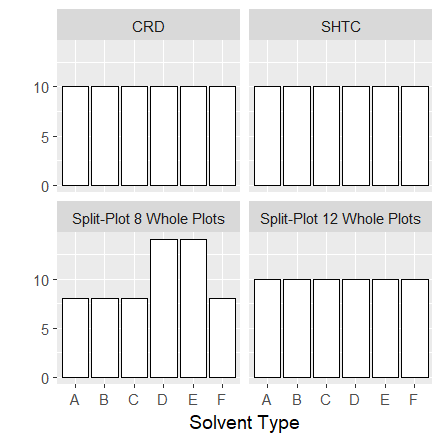
\includegraphics[width=0.475\textwidth]{ch6_barchart.png}
	}
	\caption{Frequencies of Solvent Types}
	\label{barchart1}
\end{figure}

Figure \ref{barchart1} shows that the CRD, the semi-split-plot and the split-plot design using 12 whole plots are prefectly balanced. For the split-plot design using eight whole plots it is not possible to achieve balance for the factor solvent.

\begin{figure}[!h]
	\centering{
		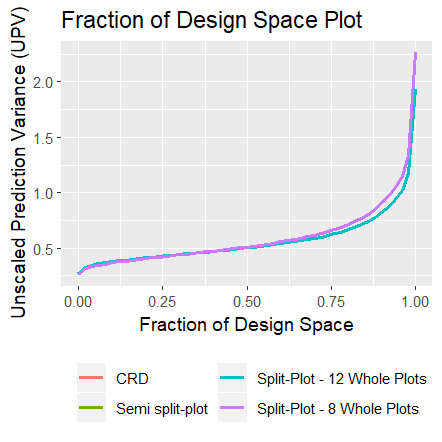
\includegraphics[width=0.475\textwidth]{ch6_fds.png}
	}
	\caption{FDS Plot}
	\label{fds}
\end{figure}

\begin{figure*}[!h]
	\centering{
		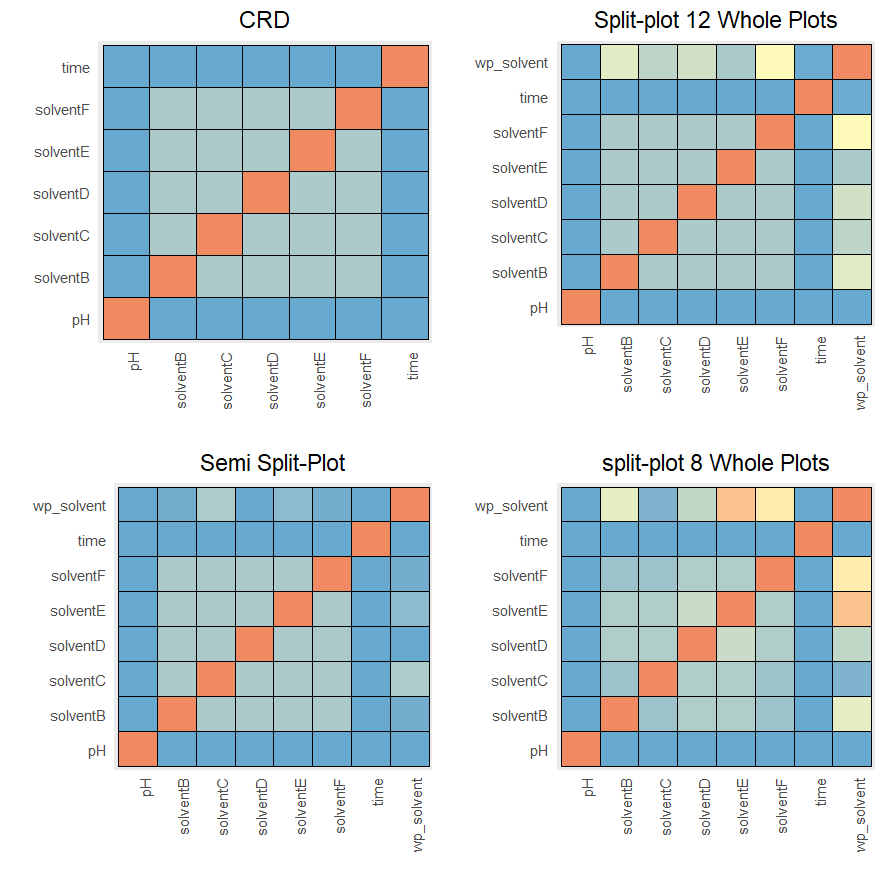
\includegraphics[width=\textwidth]{ch6_aliasingmap.png}
	}
	\caption{Correlations of Factors and Whole Plots}
	\label{heatmap1}
\end{figure*}

The aliasing heatmaps in figure \ref{heatmap1} show that there are only minor differences when comparing the designs by their inter-factor correlations. Blue cells in the figure represent low correlations while red cells are representing high correlations. All designs show some correlation in between the effects of the different solvents. The split-plot design with 8 whole plots shows a little less homogeneous correlation structure of the solvent effects. This is the result of imposing very strict restrictions to randomization.

The whole plot (\textbf{wp\_solvent} in the graph) in case of the semi split-plot design has much lower correlation with the solvent effects compared to the traditional split-plot designs.

The FDS-plot in figure \ref{fds} shows that the traditional split-plot designs with 8 whole plots performs slightly worse than the other designs in terms of prediction variance. All other designs show equal prediction variance represented by the bottom line in the graph.

Overall the semi-split-plot design is mostly equal to the CRD in terms of balance, aliasing and predictive quality. When comparing it to the split-plot designs much lower correlations of whole plot and solvent effects can be observed. Considering the practical implications of the different designs the semi-split-plot is by far the prefered solution for the given problem.

\subsection{Required Number of Whole Plots}

The previous evaluation showed that split-plot designs with SHTC-factors are not worse in terms of statistical quality than CRDs or traditional split-plots with a sufficient number of whole plots. When dealing with HTC-factors the number of whole plots is often the critical parameter. As SHTC-factors allow much more flexibility compared to true HTC-factors we are able to reduce the required number of whole plots for the given example. 

In traditional split-plot designs the required number of whole plots depends first of all on the number of HTC-factor levels. There need to be at least $l + 1$ wholeplots to be able to estimate the factor effects and the in between whole plot variation. With $l$ being the number of levels of the HTC-factor.

For SHTC-factors this is much less of a problem, as changing SHTC-factor levels inside of the whole plots is possible. Thus the minimum number of whole plots is only depending on the overall number of factor levels and the number of factor levels that can be used inside of one whole plot. All factor levels have to be used at least once. At the same time the correlation of whole plots and all other factors should be minimized to be able to estimate the model effects with high precision and avoid aliasing of whole plot effects and SHTC-factor effects.

In the following we compare semi split-plot designs for the previous example with varying number of whole plots.

\begin{figure}[!h]
	\centering{
		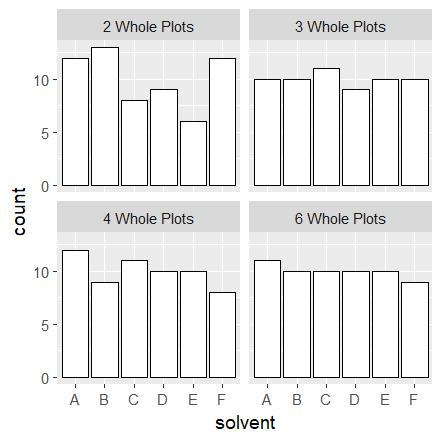
\includegraphics[width=0.475\textwidth]{ch6_barchart2.png}
	}
	\caption{Distribution of Solvent Types for Varying Numbers of Whole Plots}
	\label{barchart2} \label{balance2}
\end{figure}


Figure \ref{balance2} shows that the algorithm is not able to find a solution granting perfect balance in terms of the SHTC-factor when using only two whole plots. This problem is less severe when using three whole plots instead of just two. That statement is only true for the given example. In general the minimum number of whole plots to achieve perfect balance and minimize correlation of whole plots and the SHTC-factor depends on the size of the whole plots and on the number of possible levels in each whole plot. 

\begin{figure}[!h]
	\centering{
		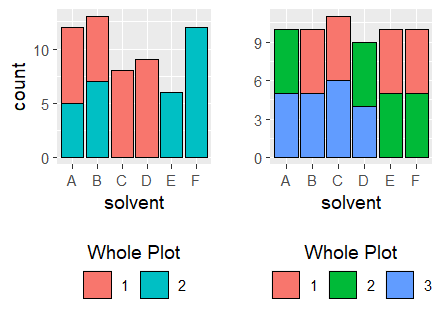
\includegraphics[width=0.475\textwidth]{ch6_barchart3.png}
	}
	\caption{Distribution of Solvent Types for 2 and 3 Whole Plots}
	\label{barchart2}
\end{figure}

The design with two whole plots shows some correlation of solvent effects and the whole plot. This correlation is reduced with every additional whole plot introduced. Going from two whole plots to three whole plots reduces the correlation a lot (see figures \ref{barchart2} and \ref{heatmap2}). Adding more whole plots does not decrease  the correlation by much. This is not a problem as the three whole plot design shows very low correlations anyways.

\begin{figure*}[!h]
	\centering{
		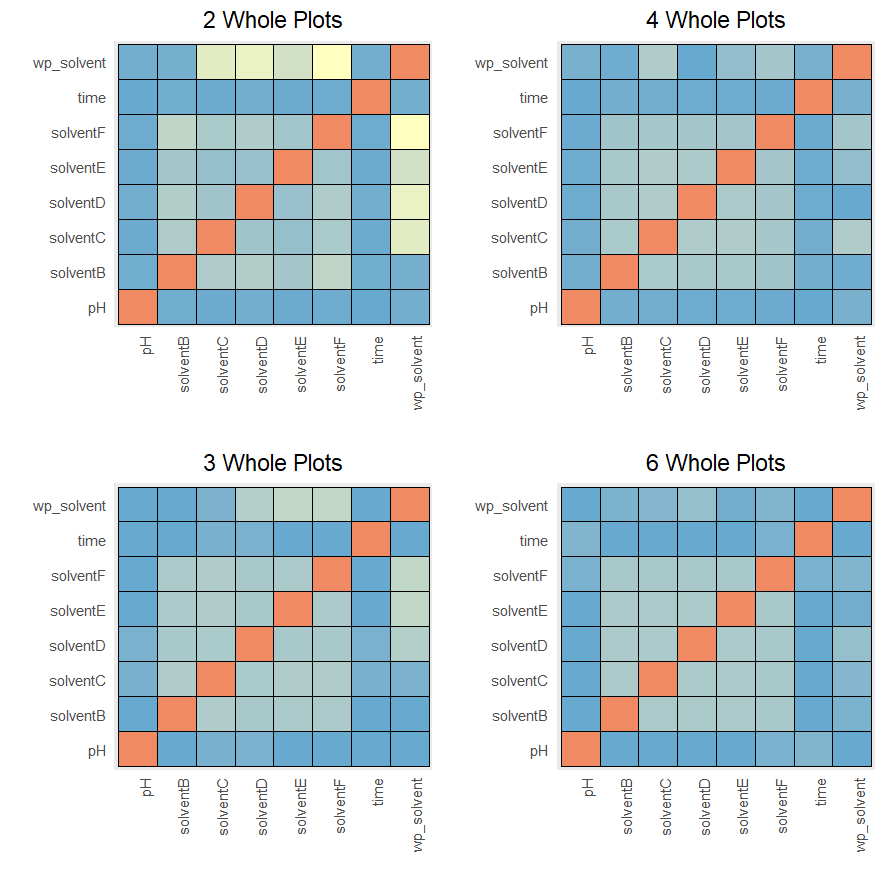
\includegraphics[width=\textwidth]{ch6_aliasing2.png}
	}
	\caption{Degree of Aliasing for Different Numbers of Whole Plots}
	\label{heatmap2}
\end{figure*}